\hypertarget{newcomer}{%
\subsection{Newcomer}\label{newcomer}}

\hypertarget{motivation}{%
\subsection{Motivation}\label{motivation}}

This pattern can help project participants be aware of the issues faced
by newcomers, and cultivate a ``beginner's mind'' themselves.

\hypertarget{context}{%
\subsection{Context}\label{context}}

When there's learning happening, it's because there is someone who is
new to a topic, or to something about the topic.

\hypertarget{forces}{%
\subsection{Forces}\label{forces}}

\begin{quote}
\Sindividuation\ \textbf{Individuation}: each person learning optimally is what's best for the community.\\
\Smutuality\ \textbf{Mutuality}: our individuality does not isolate us from one another, but draws us together.
\end{quote}

\hypertarget{problem}{%
\subsection{Problem}\label{problem}}

Newcomers can feel overwhelmed by the amount of things to learn. They
often don't know where to start. They may have a bunch of ideas that the
old-timers have never considered -- or they may think they have new
ideas, which are actually a different take on an old idea; see {{Reduce,
reuse, recycle}}. People who are new to the project can tell you what
makes their participation difficult. Since you're learning as you go as
well, you can ask yourself the same question: what aspects of this
encounter are difficult for me?

\hypertarget{solution}{%
\subsection{Solution}\label{solution}}

Instead of thinking of newcomers as ``them'', and trying to provide
solutions, we focus on newcomers as ``us'' -- which makes the search for
solutions that much more urgent. We permit ourselves to ask naive
questions. We entertain vague ideas. We add concreteness by trying {{A
specific project}}. We may then genuinely turn to others for help. We
aim to foster a culture in which the focus for everyone is on addressing
our own learning challenges rather than on ``providing'' solutions for
others {{[}1{]}}. When you begin a new project, try to systematically
take notes and gather data to analyze and reflect upon later; leave
artifacts for other future newcomers to use and build upon in their own
research. In practice this may be a lot to ask for someone just joining
a group, but over time we may have many ways to structure our collective
engagement so that it leads to research cycles based on the ``action
research'' steps \emph{reflect}, \emph{plan}, \emph{act}, and
\emph{observe}. Note that there is a parallel with the four facets
\emph{assess}, \emph{convene}, \emph{organize}, \emph{cooperate} from
Figure {[}fig:connections{]}. The history of the action research
approach, with particular emphasis on educational applications, is
surveyed in {{[}5{]}}. One method for doing the reflection/assessment
step is presented in the {{Scrapbook}} pattern. Be flexible: networked
attention (even more so than rigid cycles {{[}3{]}}) leads to new ways
of knowing and expanded access to knowledge-production {{[}7,8{]}}.

\hypertarget{rationale}{%
\subsection{Rationale}\label{rationale}}

A newcomer's confusion about how best to get involved or what the point
of all this actually is may be due to a lack of structure in the project
{{Roadmap}}. Sharing vulnerability and confusion gives us a chance to
learn.

\hypertarget{resolution}{%
\subsection{Resolution}\label{resolution}}

An awareness of the difficulties that newcomers face can help us be more
compassionate to ourselves and others. We strengthen the community by
supporting all participants' \textbf{individuation}. We have a better
chance of making the project useful for others if we're clear about how
it is useful to \emph{us}. By welcoming newcomers, we enhance the sense
of \textbf{mutuality} with people who have never encountered the project
before, and learn together with them. The facts start to become useful
when we understand how people perceive them {{[}4{]}}.

\hypertarget{example-1}{%
\subsection{Example 1}\label{example-1}}

Wikipedia {{Newcomers}} can make use of resources that include a
``Teahouse'' where questions are welcomed, a platform extension that
changes the user interface for new editors, and lots of
documentation.\footnote{\url{https://en.wikipedia.org/wiki/Wikipedia:Teahouse}},\footnote{\url{https://en.wikipedia.org/wiki/Wikipedia:GettingStarted}},\footnote{\url{https://en.wikipedia.org/wiki/Help:Editing}}
exceptional newcomers may be given special recognition.\footnote{\url{https://en.wikipedia.org/wiki/Template:The_New_Editor\%27s_Barnstar}}
interest to the Wikimedia Foundation.\footnote{\url{https://meta.wikimedia.org/wiki/Research:Newcomer_survival_models}}
However, ``Nearly all editors begin with a burst of activity, then
quickly tail off'' {{[}6{]}}. The degree to which those editors who are
retained strive to maintain a ``beginner's mind'' is less clear. As
regards learning their way around the community, there is quantitative
support {{[}6{]}} for the claim that ``novice users learn the rules and
conventions for contributing both through observation and direct
coaching from more knowledgeable others'' {{[}2{]}}.

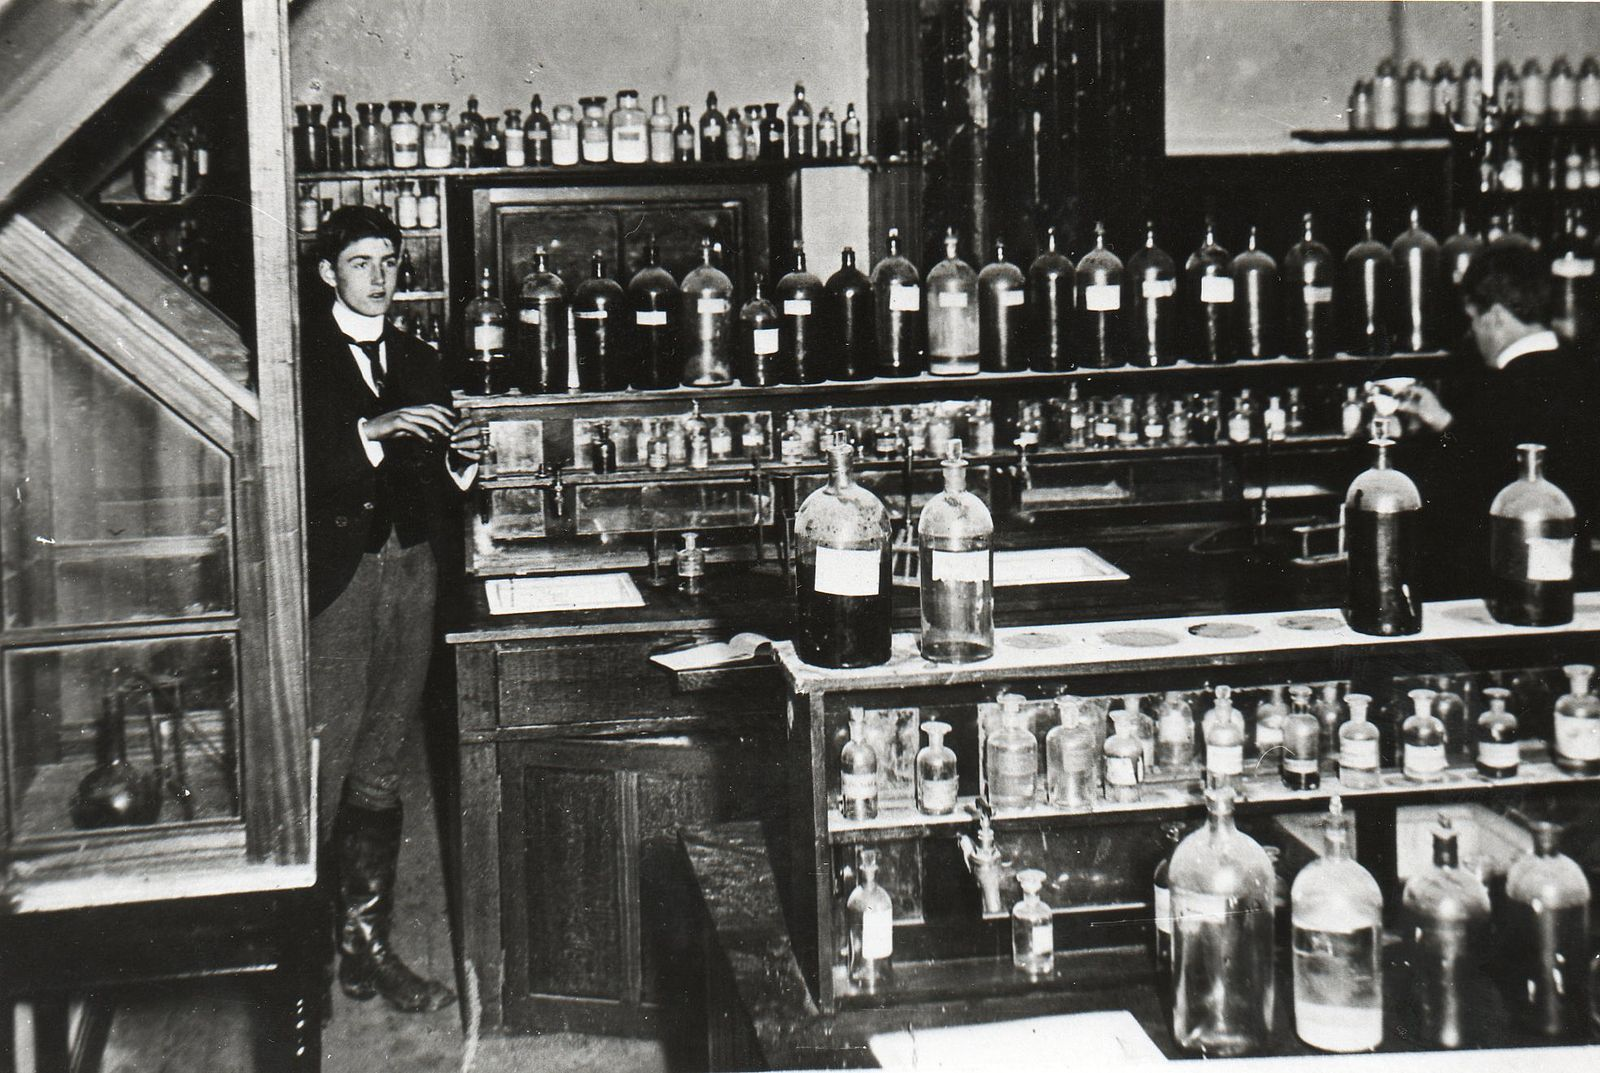
\includegraphics{images/The_Science_Laboratory.jpg}\\
\emph{Science Hall: Aspatria Agricultural College, Aspatria, Cumberland,
UK}

\hypertarget{example-2}{%
\subsection{Example 2}\label{example-2}}

It will often be pragmatic to connect {{Newcomers}} with employment
directly, so that the future university may see a closer coupling of
science and industry than would be found in the old Science Hall.
Inspiration can be drawn the London-based freelancing cooperative
Founders\&Coders, which is able to offer intensive training in web
development at no cost to successful applicants, on the basis that some
trainees will choose to join the cooperative as paying members later
on.\footnote{\url{http://www.foundersandcoders.com/academy/}}

\hypertarget{whats-next-in-the-peeragogy-project}{%
\subsection{What's Next in the Peeragogy
Project}\label{whats-next-in-the-peeragogy-project}}

More detailed guides can show {{Newcomers}} how they can contribute and
what to expect when they do. We should have different guides for
different ``user stories''. We can start by listing some of the things
we're currently learning about.

\hypertarget{references}{%
\subsection{References}\label{references}}

\begin{enumerate}
\def\labelenumi{\arabic{enumi}.}
\item
  D. Boud and A. Lee. 2005. ``Peer learning'' as pedagogic discourse for
  research education. \emph{Studies in Higher Education} 30, 5:
  501--516.
\item
  Susan L Bryant, Andrea Forte, and Amy Bruckman. 2005. Becoming
  Wikipedian: Transformation of participation in a collaborative online
  encyclopedia. \emph{Proceedings of the 2005 international aCM sIGGROUP
  conference on supporting group work}, ACM, 1--10.
\item
  Y. Engeström. 1999. Innovative learning in work teams: Analyzing
  cycles of knowledge creation in practice. In \emph{Perspectives on
  activity theory}, Yrjö Engeström, Reijo Miettinen and Raija-Leena
  Punamäki (eds.). Cambridge University Press, 377--406.
\item
  Paulo Freire. 1982. Creating alternative research methods: Learning to
  do it by doing it. In \emph{Creating knowledge: A monopoly}, B. Hall,
  A. Gillette and R. Tandon (eds.). Society for Participatory Research
  in Asia, 29--37.
\item
  Jean McNiff. 2013. \emph{Action research: Principles and practice}.
  Routledge.
\item
  Katherine Panciera, Aaron Halfaker, and Loren Terveen. 2009.
  Wikipedians are born, not made: A study of power editors on Wikipedia.
  \emph{Proceedings of the aCM 2009 international conference on
  supporting group work}, ACM, 51--60.
\item
  Gilbert Simondon. 2012. Technical mentality. In \emph{Gilbert
  Simondon: Being and technology}, Arne De Boever, Alex Murray, Jon
  Roffe and Ashley Woodward (eds.). Oxford University Press, 1--15.
\item
  C.S. Wagner. 2008. \emph{The new invisible college: Science for
  development}. Brookings Inst Press.
\end{enumerate}

\begin{center}\rule{0.5\linewidth}{0.5pt}\end{center}
